\documentclass{beamer}
\usepackage{xcolor}
\usepackage[utf8]{inputenc}
\usepackage[english]{babel} 
\usepackage{listings}
\usepackage{amsmath}
\usepackage{algorithm}
\usepackage[noend]{algpseudocode}
\algdef{SE}[DOWHILE]{Do}{doWhile}{\algorithmicdo}[1]{\algorithmicwhile\ #1}%
\algnewcommand{\LineComment}[1]{\State \(\triangleright\) #1}

%\usepackage{algorithmic}
%\algnewcommand{\LineComment}[1]{\State \(\triangleright\) #1}

\usepackage{parcolumns}


\usetheme{Madrid}
\usecolortheme{beaver}

\beamertemplatenavigationsymbolsempty

\renewcommand{\emph}{\textcolor{red}}

%------------------------------------------------------------\usepackage{amsmath,amssymb,amsthm,algorithmic,algorithm}
%This block of code defines the information to appear in the
%Title page
\title[Resource Sharing] %optional
{Enabling resource sharing in dataflow circuits}

\author[Marmet] % (optional)
{Axel Marmet}

\institute[EPFL] % (optional)

\date[2020] % (optional)

\begin{document}

%The next statement creates the title page.
\frame{\titlepage}


\begin{frame}
\frametitle{Table of Contents}
\tableofcontents
\end{frame}

\section{Introduction}
\begin{frame}{Dataflow Circuits}
    \begin{columns}[T]
    \begin{column}{0.45\textwidth}
        Dataflow circuits are latency-insensitive circuits where the data is represented by tokens and components communicate using handshakes. \\
       The components are grouped into BBs (Basic Blocks) connected by control flow edges; when a BB is triggered, all components inside it are executed
    \end{column}
    \begin{column}{0.45\textwidth}
        \begin{center}
      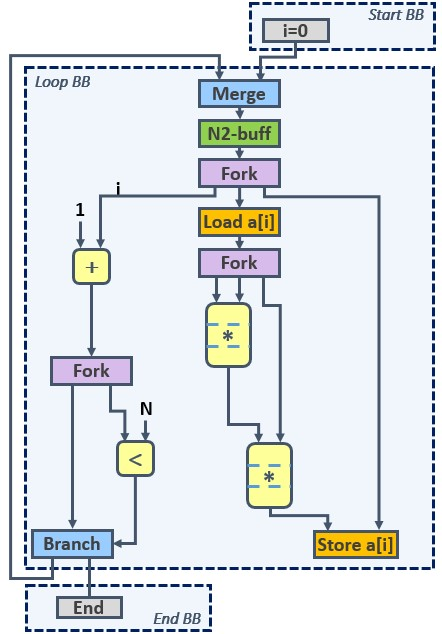
\includegraphics[scale=0.35]{datflow_example.jpg}
      Example from Josipovic et al\footnotemark
    \end{center}
    \end{column}
  \end{columns}
        \footnotetext{Josipovic et al., Buffer placement and sizing for high-performance dataflow circuits, FPGA'20}
\end{frame}
\begin{frame}{Resource sharing}
    There are two problems when sharing resources
    \begin{enumerate}
        \item Finding where to share, hard because there is no predetermined schedule
        \item Share in a way that ensures correct and deadlock-free execution
    \end{enumerate}
\end{frame}
\section{Motivation}
\begin{frame}{Prerequisite information}
    We define occupancy as the amount of tokens a component holds in steady state divided by the maximum number of tokens it can hold. We already know how to obtain this value\footnotemark.
    \begin{columns}[T]
    \begin{column}{0.45\textwidth}
        \begin{center}
      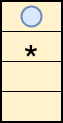
\includegraphics[scale=0.25]{occupancy_25.png} \\
                Multiplier with occupancy $0.25$ 
    \end{center}    \end{column}
    \begin{column}{0.45\textwidth}
 \begin{center}
      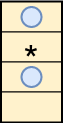
\includegraphics[scale=0.25]{occupancy_50.png} \\
        Multiplier with occupancy $0.5$ 
    \end{center}
    \end{column}
  \end{columns}
      \footnotetext{Josipovic et al., Buffer placement and sizing for high-performance dataflow circuits, FPGA'20}
\end{frame}
\begin{frame}[fragile]
\frametitle{Motivation}
\begin{columns}[T]
    \begin{column}{0.45\textwidth}
      \begin{itemize}
          \item New iteration every two clock cycles
          \item Each multiplier has an occupancy of $0.5$
          \item Using only one multiplier would not hurt performance but diminish size of circuit
      \end{itemize}
    \end{column}
    \begin{column}{0.45\textwidth}
        \begin{center}
      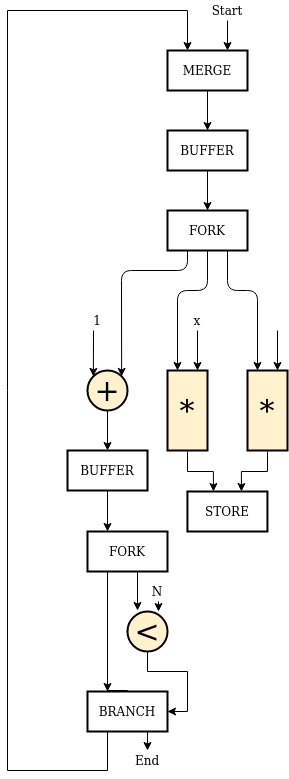
\includegraphics[scale=0.25]{base_case.png}
    \end{center}
    \end{column}
  \end{columns}
\end{frame}

\newcommand{\initialAnimation}[1]{
\begin{frame}{Initial idea}
\begin{columns}[T]
    \begin{column}{0.45\textwidth}
    We add two new components to enable sharing \newline \newline
    \emph{Selector} \newline
    Responsible for selecting inputs in a way that ensures fairness and will never deadlock. 
    \newline 
    \newline
    \emph{Distributor} \newline
    Must send the resulting token to the correct outputs, is told where to send by the Selector through a FIFO.
    \end{column}
    \begin{column}{0.45\textwidth}
        \begin{center}
      \includegraphics[scale=0.25]{#1}
    \end{center}
    \end{column}
  \end{columns}
\end{frame}
}

\initialAnimation{animation_tehb_0.png}
\initialAnimation{animation_initial_1.png}
\initialAnimation{animation_initial_2.png}
\initialAnimation{animation_initial_3.png}
\initialAnimation{initial_animation_4.png}
\initialAnimation{initial_animation_5.png}

\section{Deadlock avoidance}
\newcommand{\tehbAnimation}[1]{
\begin{frame}{Necessary transparent buffer in distributor}
    \begin{columns}[T]
    \begin{column}{0.45\textwidth}
    The distributor being able to hold the outputs is sometimes essential to allow the continuation of the computation. We enable this by using a 1 slot transparent buffer (TEHB)
    \end{column}
    \begin{column}{0.45\textwidth}    
    \begin{center}
      \includegraphics[scale=0.25]{#1}
    \end{center}
    \end{column}
  \end{columns}
\end{frame}
}

\tehbAnimation{animation_tehb_0.png}
\tehbAnimation{animation_tehb_1.png}
\tehbAnimation{animation_tehb_2.png}
\tehbAnimation{animation_tehb_3.png}


%TODO add animation
\begin{frame}{Deadlock avoidance}
  How to schedule execution without causing deadlock ?
  \begin{columns}[T]
    \begin{column}{0.25\textwidth}
        \begin{center}
      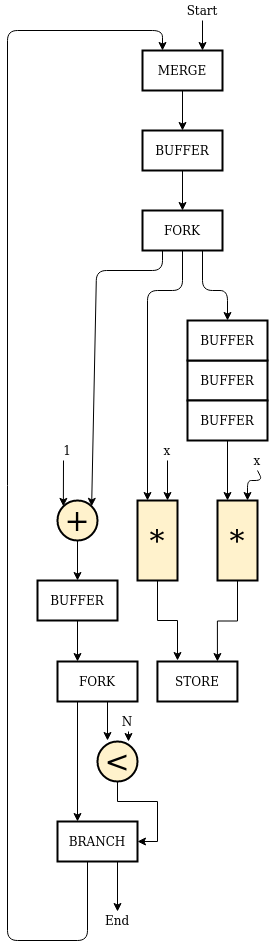
\includegraphics[scale=0.25]{blocking_unshared.png}
    \end{center}
    \end{column}
    \begin{column}{0.1\textwidth}
    \begin{center}
        becomes
    \end{center}
    \end{column}
    \begin{column}{0.25\textwidth}
        \begin{center}
      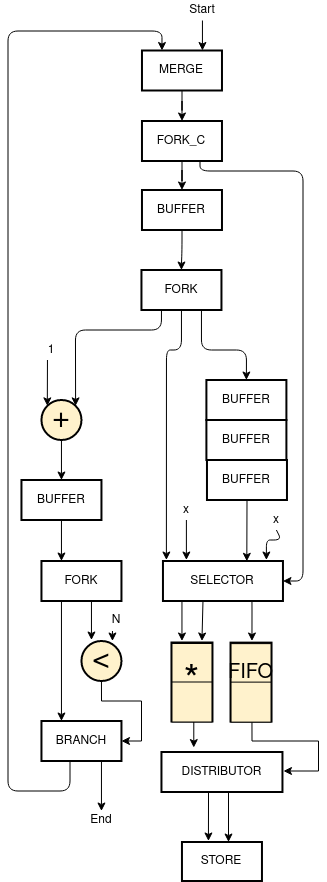
\includegraphics[scale=0.23]{deadlock_1.png}
    \end{center}
    \end{column}
  \end{columns}
\end{frame}

\newcommand{\deadlockAnimation}[1]{
\begin{frame}{Deadlock avoidance}
\begin{center}
\includegraphics[scale=0.25]{#1}
\end{center}
\end{frame}
}

\deadlockAnimation{deadlock_2.png}
\deadlockAnimation{deadlock_3.png}
\deadlockAnimation{deadlock_4.png}
\deadlockAnimation{deadlock_5.png}
\deadlockAnimation{deadlock_6.png}
\deadlockAnimation{deadlock_7.png}



\begin{frame}{Ordering}
\emph{Among BBs} \\
We must ensure that all shared computations from a BB must happen before other shared computations start \newline \newline
\emph{Per BB} \\
We will also enforce an ordering among computations in the same BB. Although not strictly necessary it makes the sharing easier to model to the MILP.
\end{frame}

\begin{frame}{Modelling sharing to the MILP}
Two possibilities
\begin{enumerate}
    \item Modify shared components's latencies and initiation intervals
    \item Implement sharing using dataflow components
\end{enumerate}
\end{frame}

\begin{frame}{Modelling using latency and II}
      \begin{columns}[T]
    \begin{column}{0.25\textwidth}
        \begin{center}
      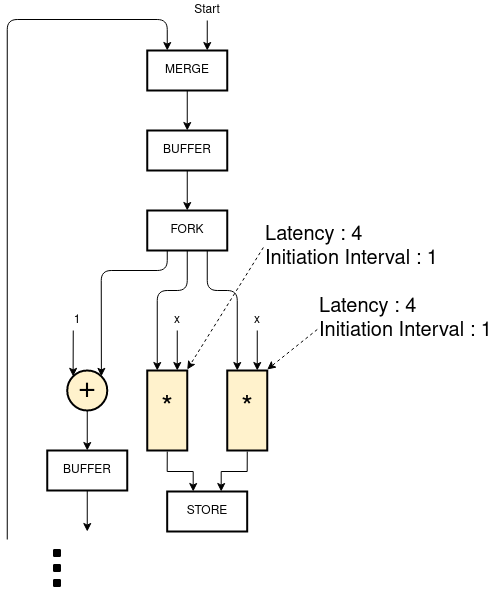
\includegraphics[scale=0.25]{latency_unshared.png}
    \end{center}
    \end{column}
    \begin{column}{0.1\textwidth}
    \begin{center}
        becomes
    \end{center}
    \end{column}
    \begin{column}{0.25\textwidth}
        \begin{center}
      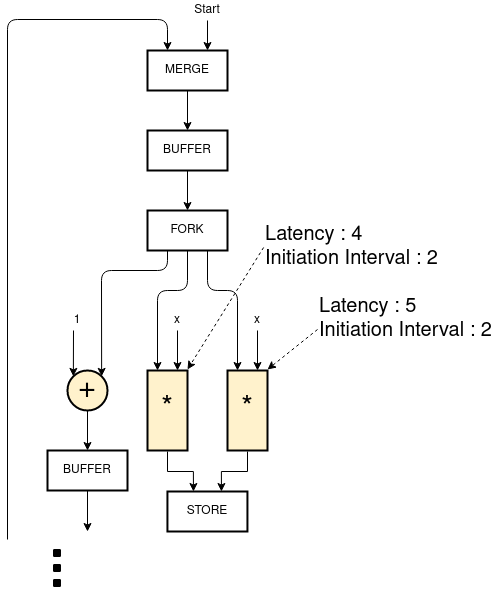
\includegraphics[scale=0.25]{latency_shared.png}
    \end{center}
    \end{column}
  \end{columns}
\end{frame}

\begin{frame}{Disadvantage of latency and II}
    \begin{columns}[T]
    \begin{column}{0.45\textwidth}
We ended up choosing the dataflow components approach because updating latencies depends on buffer placement elsewhere in the dataflow circuits. For example latency does not need to be increased in the shown dataflow circuit due to the supplementary buffer.    
    \end{column}
    \begin{column}{0.45\textwidth}
    \begin{center}
     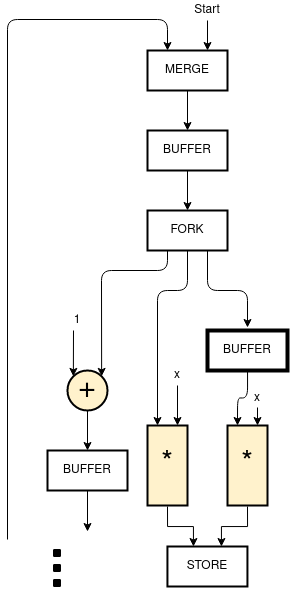
\includegraphics[scale=0.28]{latency_with_buffer.png}
    \end{center}
    \end{column}
\end{columns}
\end{frame}

\begin{frame}{Modelling using dataflow components}
    \begin{columns}[T]
    \begin{column}{0.3\textwidth}
    We use the control path of the BB to enforce an ordering
    \end{column}
    \begin{column}{0.45\textwidth}
        \begin{center}
      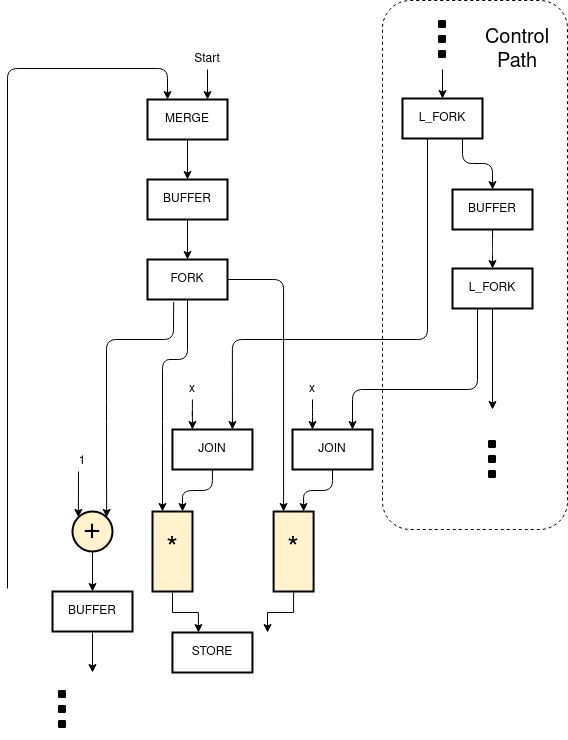
\includegraphics[scale=0.25]{dataflow_shared.png}
    \end{center}
    \end{column}
  \end{columns}\end{frame}

\begin{frame}{Model vs reality}
Using additional components is great for modelling sharing but actually implementing like it would become quite costly due to the amount of lazy forks and buffers. As such we show how we get from the simple but costly way of sharing to the more optimized one.
\end{frame}

\section{Components}
\begin{frame}{Given to the MILP}
\begin{center}
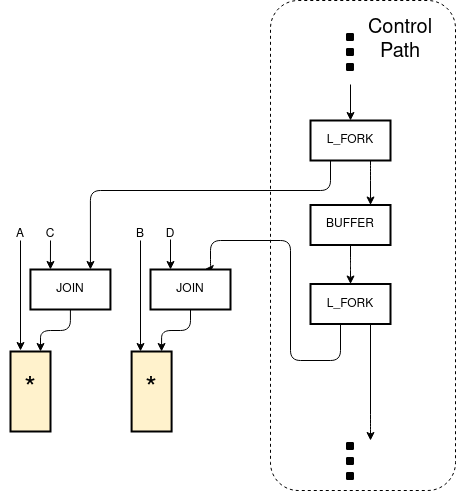
\includegraphics[scale=0.4]{given_to_milp.png}
\end{center}
\end{frame}

\begin{frame}{Unoptimized component}
One lazy fork necessary per shared component.
\begin{center}
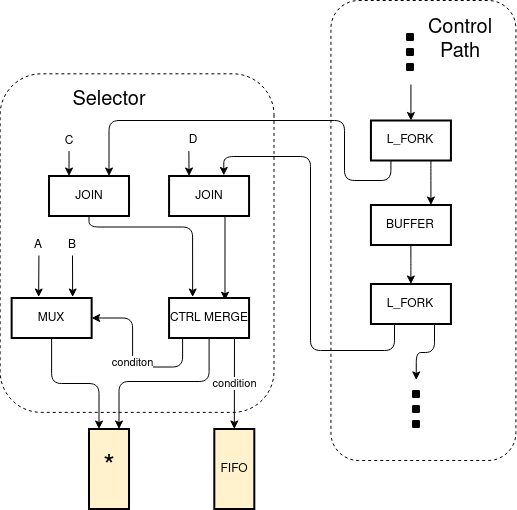
\includegraphics[scale=0.4]{simple_selector.png}
\end{center}
\end{frame}

\begin{frame}{Optimized component}
One lazy fork necessary per BB.
\begin{center}
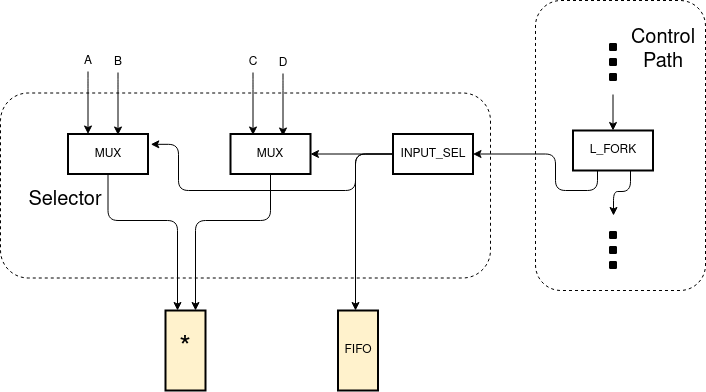
\includegraphics[scale=0.35]{opti_selector.png}
\end{center}
\end{frame}

\begin{frame}{INPUT SEL}
\begin{center}
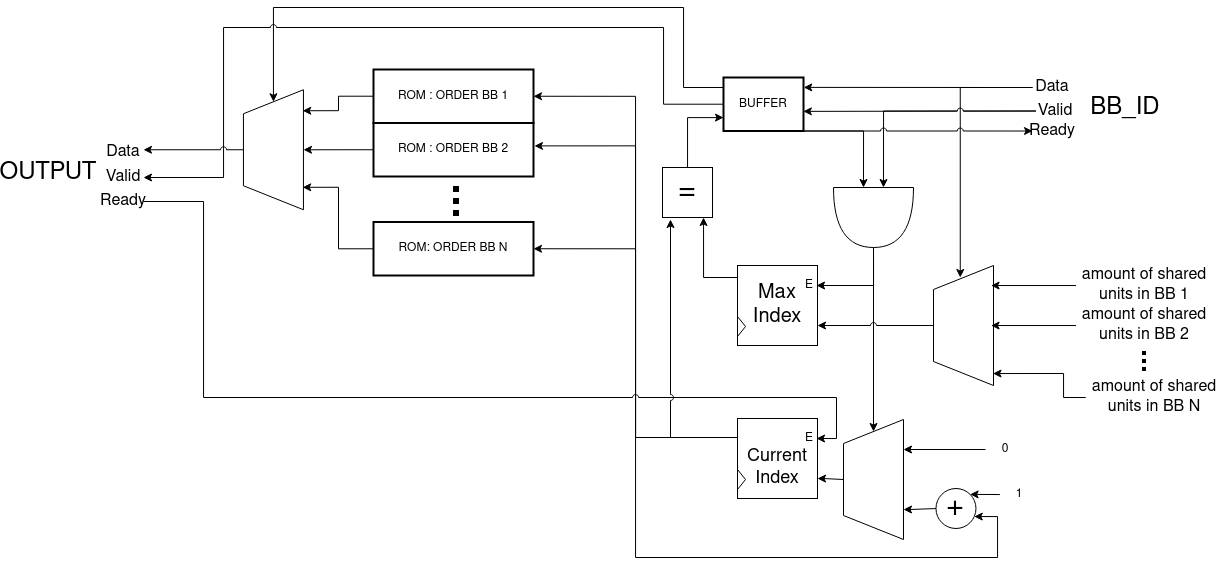
\includegraphics[scale=0.27]{SEL_INPUT.png}
\end{center}
\end{frame}

\begin{frame}{Full system}
\begin{center}
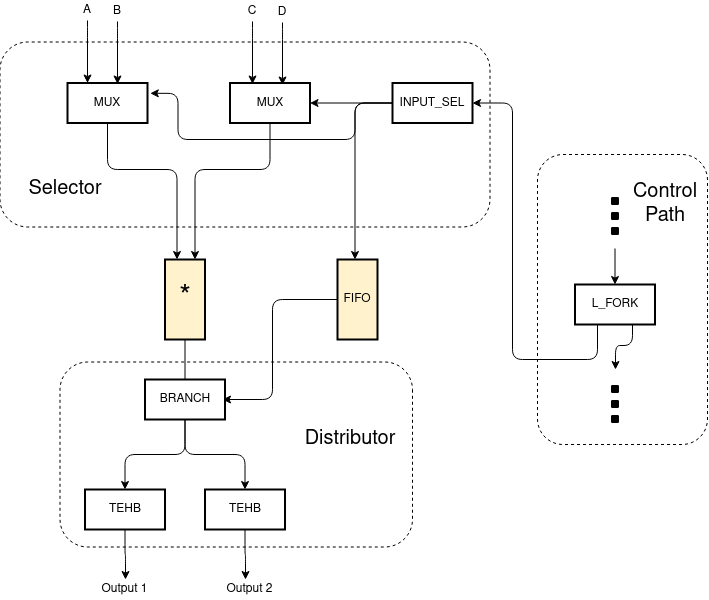
\includegraphics[scale=0.3]{full_example.png}
\end{center}
\end{frame}

\section{Algorithm}
\begin{frame}{Algorithm}
\begin{columns}

\end{columns}
    \begin{columns}[T]
    \begin{column}{0.45\textwidth}
We are given the disjoint set information that we use exhaustively in our algorithm by Josipovic et al., Buffer placement and sizing for high-performance dataflow circuits, FPGA'20
\end{column}
    \begin{column}{0.45\textwidth}
    \begin{center}
     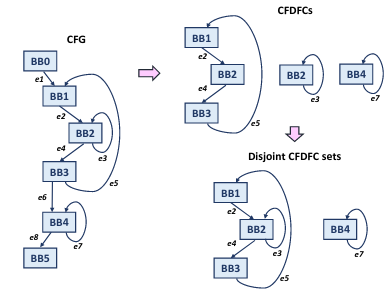
\includegraphics[scale=0.4]{input_algorithm.png}
    \end{center}
    \end{column}
\end{columns}
\end{frame}

\begin{frame}[fragile]{Algorithm}
 \small
 \scriptsize
\begin{algorithmic}[1]
    \LineComment intra-set
    \For{s $\in$ disjoint\_sets}
        \For{mg $\in$ marked\_graphs}
            \State merge\_groups = $\{ n \mid n \in s, is\_shareable(n)\}$
            \Do
                \For{$g_1, g_2 \in merge\_groups, g_1 \neq g_2$}
                    \If{$ g_1.occupancy + g_2.occupancy \leq 1$}
                        \For{ ord $\in$ possible\_orderings$(g_1 \cup g_2)$}
                            \LineComment we use the MILP here
                            \If{$does\_not\_affect\_throughput(ord)$}
                                \State merge\_groups.update($g_1, g_2, g_1 \cup g_2, ord$) 
                            \EndIf
                        \EndFor
                    \EndIf
                \EndFor
            \doWhile{merge\_groups changed}
            \State s.add(merge\_groups)
        \EndFor
    \EndFor
    \algstore{myAlgo}
\end{algorithmic}
\end{frame}

\begin{frame}[fragile]{Algorithm}
 \small
 \scriptsize
\begin{algorithmic}[1]
    \algrestore{myAlgo}
    \LineComment inter-set
    \State global\_merge\_groups = \{\}
    \For{$s \in disjoint\_sets$}
        \State i = 0;
        \For{$merge\_group \in s$}
            \State global\_merge\_groups($i++$).add(merge\_group)
        \EndFor
    \EndFor
    
    \LineComment extra-set
    \For{$n \in \{ n \mid n \in nodes,  \neg\exists s \in disjoint\_set :\, n \in s \}$ }
        \State global\_merge\_groups(random\_index).add(n)
    \EndFor
\end{algorithmic}
\end{frame}

\section{Next steps}
\begin{frame}{Next steps}
\begin{itemize}
    \item Test the current flow
    \item Find a heuristic or algorithm to find best ordering without exhaustive search
    \item Get quantitative results
\end{itemize}
\end{frame}

\end{document}